
\begin{figure*}
  \centering

\begin{subfigure}[b]{\textwidth}
\centering
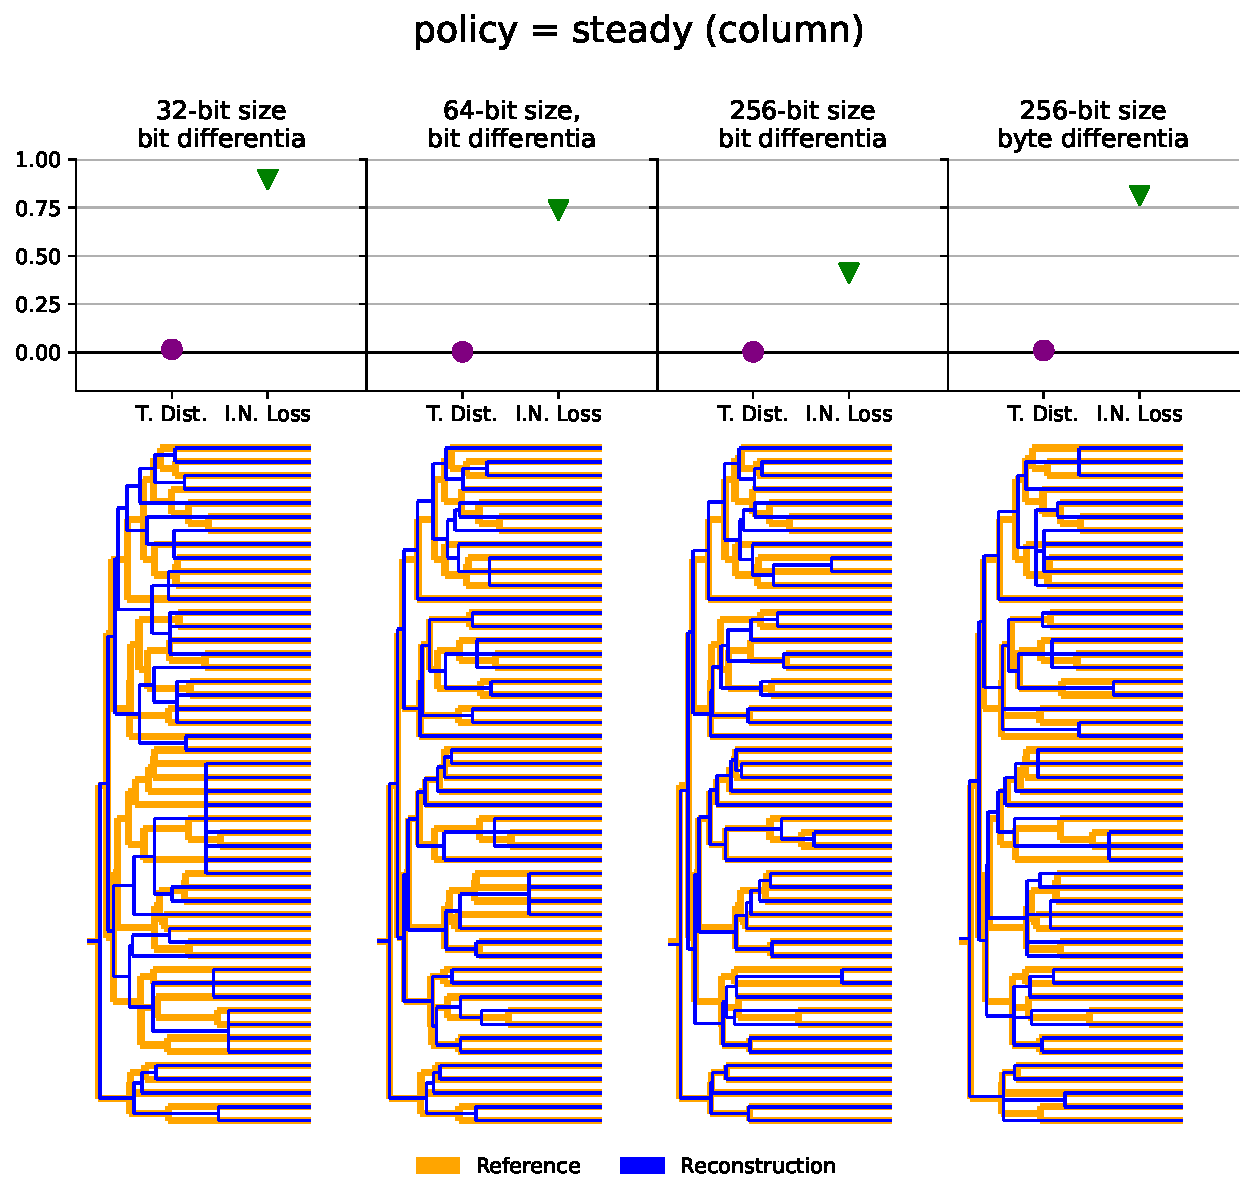
\includegraphics[width=0.5\textwidth]{binder/binder/outplots/a=examplepanel+policy=col-steady+regime=drift+ext=}%
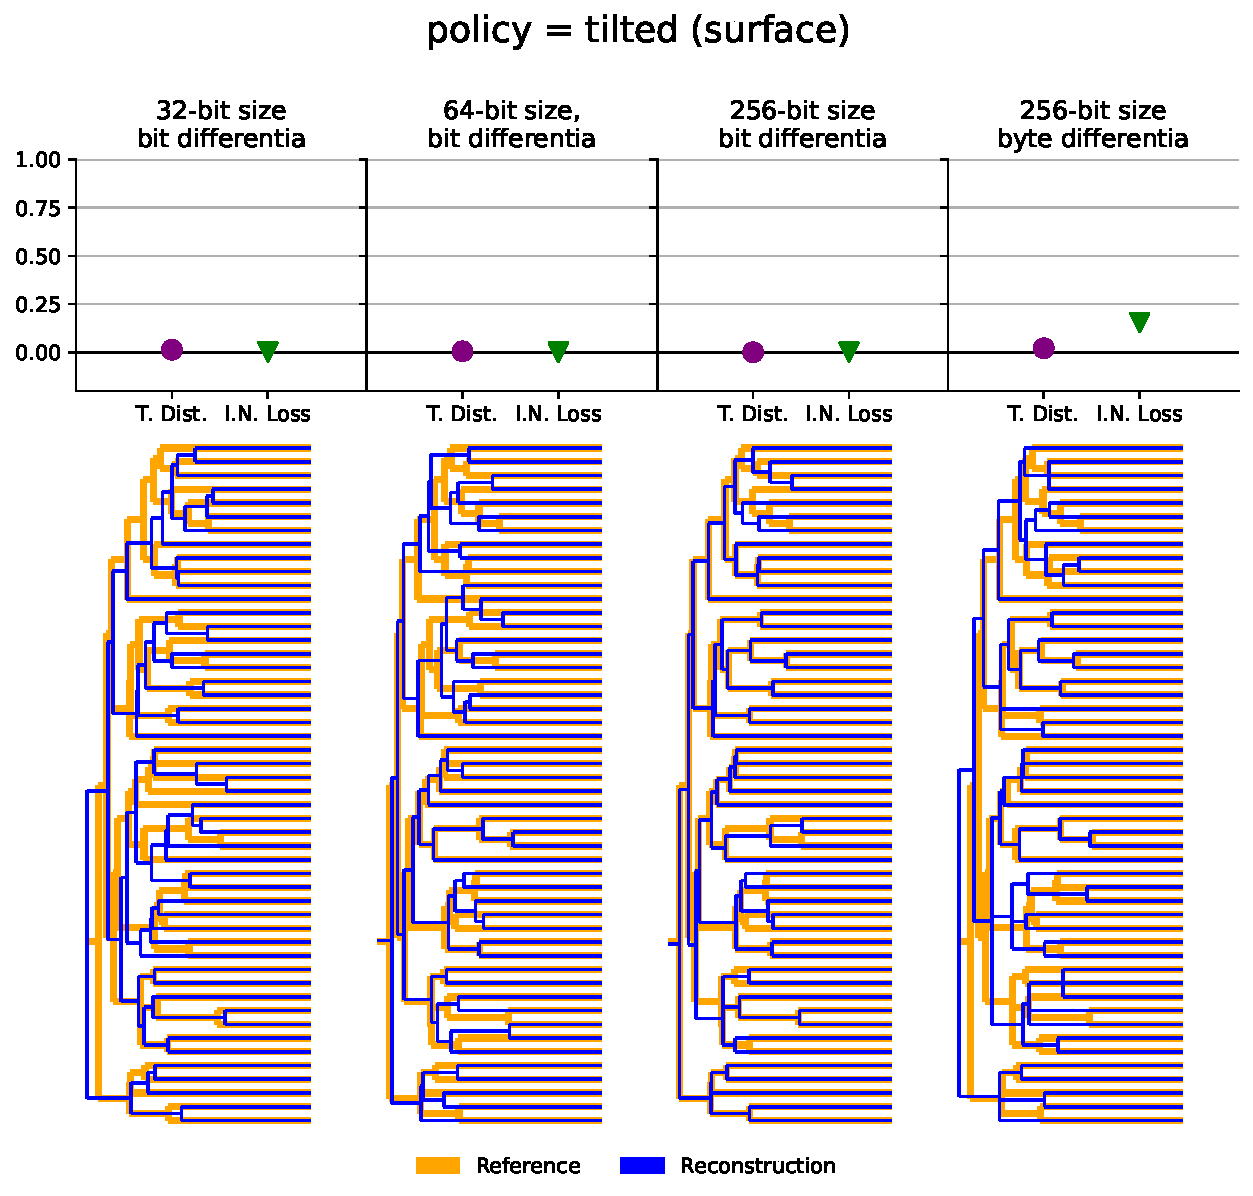
\includegraphics[width=0.5\textwidth]{binder/binder/outplots/a=examplepanel+policy=surf-tilted+regime=drift+ext=}
\caption{\textbf{drift regime} --- high phylogenetic richness}
\label{fig:examplepanel-drift}
\end{subfigure}

\begin{subfigure}[b]{\textwidth}
\centering
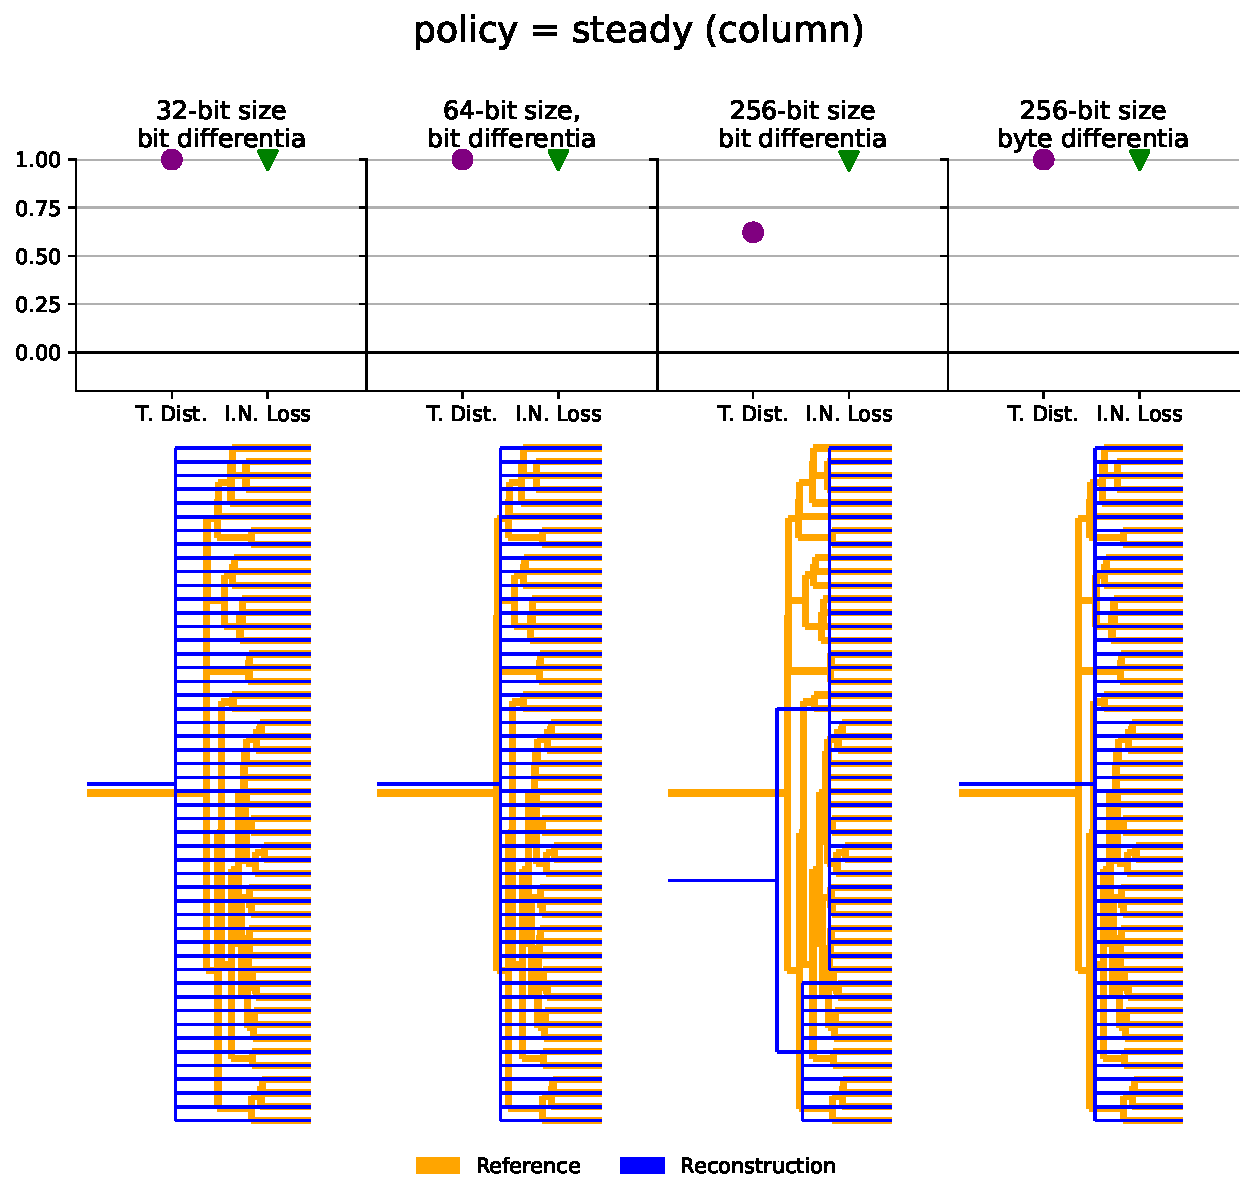
\includegraphics[width=0.5\textwidth]{binder/binder/outplots/a=examplepanel+policy=col-steady+regime=plain+ext=}%
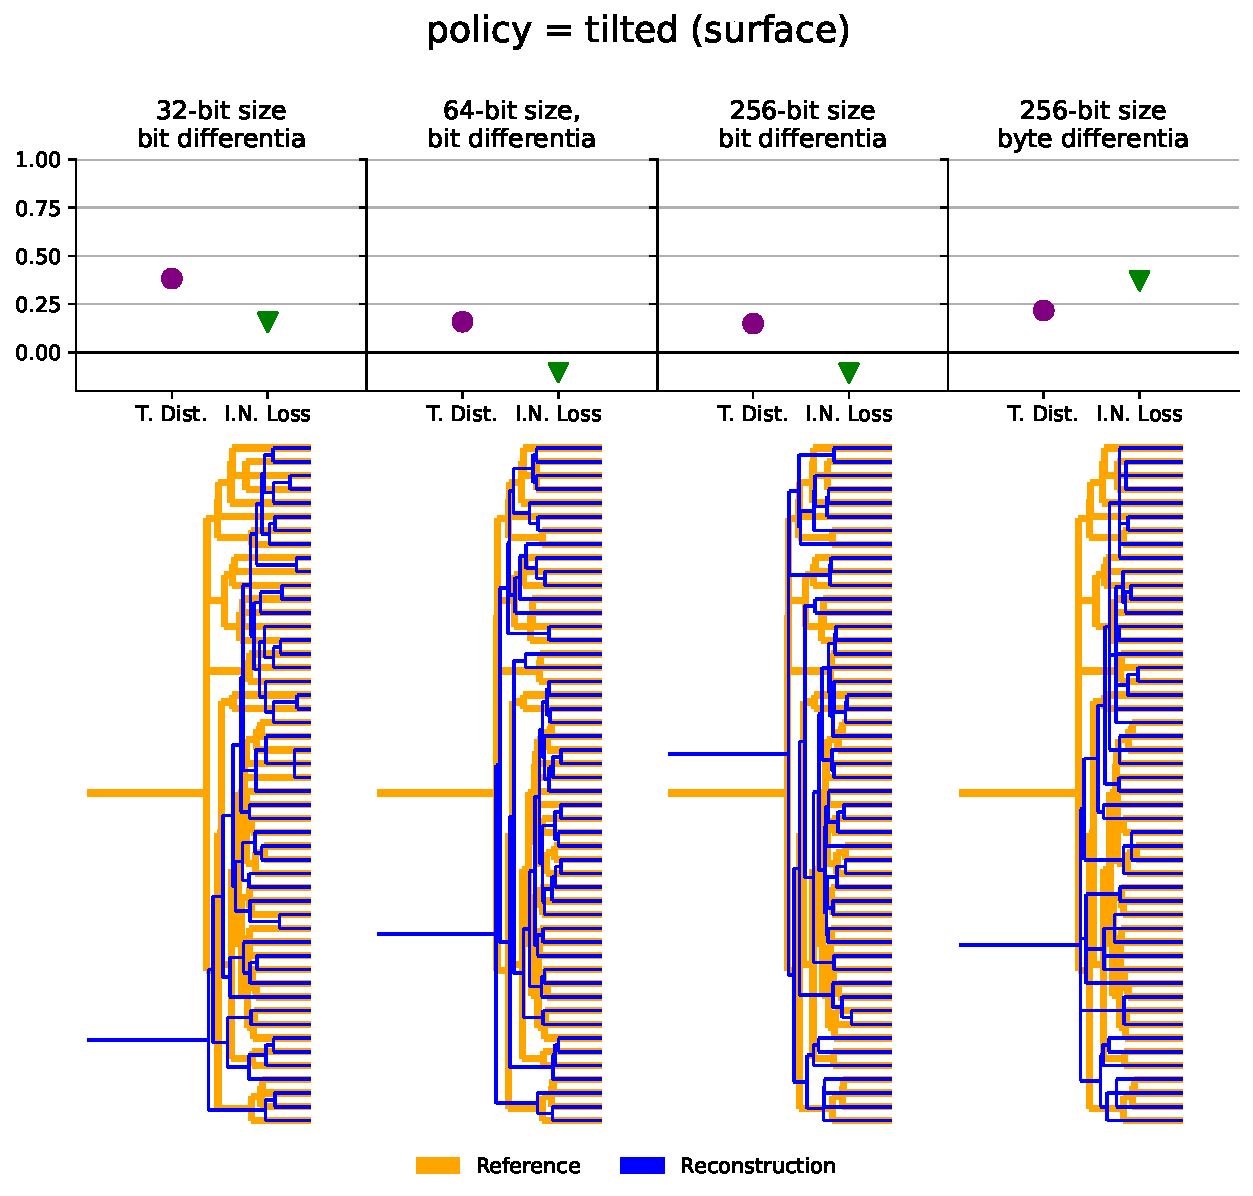
\includegraphics[width=0.5\textwidth]{binder/binder/outplots/a=examplepanel+policy=surf-tilted+regime=plain+ext=}
\caption{\textbf{plain regime} --- low phylogenetic richness}
\label{fig:examplepanel-plain}
\end{subfigure}

  \caption{%
  \textbf{Example Phylogeny Reconstructions and Quality Metric Assessments.}
  \footnotesize
  Comparison of reconstruction to reference tree for steady and tilted policies under drift (\ref{fig:examplepanel-drift}) and plain (\ref{fig:examplepanel-plain}) evolutionary regimes.
  Panel tops show reconstruction quality metrics (triplet distance and inner node loss) and panel bottoms overlay reconstruction (blue) on reference tree (orange).
  Left panels are steady policy and right panels are tilted policy.
  Phylogeny time axes are log scale.
  Note that overlay layout is naive, so can underrepresent agreement between trees; however, comparison is informative to general differences in tree structure.
  Steady policy causes catastrophic comb polytomies in plain regime, where most recent common ancestor among taxa is very recent.
  Steady policy also experiences notable inner node loss under phylogenetically-rich drift scenario, but effect on triplet distance is negligible.
  In all cases, byte differentia configurations have higher, or comparable, triplet distance and inner node loss than correspondingly sized bit differentia configuration.
  }
  \label{fig:examplepanel}

\end{figure*}
